\section{Abstract}

How to design disaggregated data structures is an open problem. This document
studies design decisions which may improve hash table performance.

\section{Introduction}

Far memory data structures are difficult to work with, especially when the
structures are shared by many processes. Obtaining serialization of operations
can be expensive and slow when using only one sided operations. The issue is
that when operations conflict clients need to retry their failed operations.
This requires multiple round trips, and often reads and writes. Ideally
operations can succeed in the common cases, and when conflicts do occur they can
be cleaned up later. Our model of disaggregation is at the level of a single
rack, where all of the machines are connected by a programmable switch. The
switch has a perfect view of all the racks traffic and can modify the traffic in
flight.

\section{Existing Hash Tables}

Clover~\cite{clover} and RACE~\cite{race}, are the only hash tables designed
specifically with disaggregation in mind. Clover supports read and write
operations on keys, writes append to a linked list, the tail of the list is the
keys current address for reads. Clover is lockless, but does not readily support
inserts and deletes at the rate that it supports reads and writes. RACE supports
inserts, deletes, reads and writes, but it does so at significant costs to the
application.

\textbf{load balancing:} Race uses power of 2 hashing on inserts. It selects the
location which has the lowest load. While this prevents load imbalance, reads
need to read two indexes rather than one. Further concurrent inserts are not
safe by their description if two concurrent writes occur and land in different
hash buckets one must be deleted. This requires an additional read after each write.

\textbf{Space:} Race uses associative hashing for each bucket. Each key can
therefore land in at most 16 locations. This fact prevents inserts from failing
in the common case, however on reads all 16 slots must be read.

\textbf{CAS size:} CAS operations are 64 bits. Therefore all race atomic entries
are pinned to 64 bit size. 48 bits of the 64 are used as an address offset, the
other 16 are used half for the size of the key, and the other half is used as a
hash of the key. THis means that writes can only take place in 255 sizes, and
that we cannot verify that the key is correct until the data is read from the
hash table. Ideally we could ensure that hash entry is correct with a single lookup.

\textbf{Self Verifying Data:} Clover ensure reads are valid by inspecting a null
pointer at the end of the write chain. In race the head pointer must be read,
and then the data must be traversed too for each read. This means that in RACE
all lookups require two round trips.

\section{Potential Extensions}:

Here we propose three structures. First a write unit with a simple
implementation which allows for simple append operations to sequential memory
addresses. Using this structure we propose a hash index, and hash table data
structure. In all cases the data structures are designed to enable a switch
without relying on one to do so.

\subsection{Write Unit}:

\begin{figure}[t] 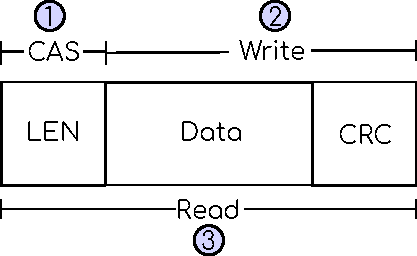
\includegraphics[width=0.485\textwidth]{fig/WriteBufEntry.pdf}
%  \vskip -0.5em
\caption{Individual Entry. Entries are allocated by executing CAS operations
with the entry's length. If the CAS completes the entry is allocated. The body
of the entry is filled by a traditional write. Reads are async and can se
partially written data. A write entry is valid only once it can be read in it's
entirety with a valid CRC}

\label{fig:write_unit}
%      \vskip -0.5em
\end{figure}

\textbf{CAS as allocate} In Clover and RACE data is written first, and once
completed a CAS is issued which points to write. We opt instead for using CAS as
an allocate, rather than commit operation. The CAS specifies the size of the
entry to be written following the CAS in sequential memory. This approach is
used in log structured file systems, and is the core of Black-Box
Numa~\cite{black-box-numa}.  This approach has the advantage of enabling all
writes to occur sequentially in memory. The disadvantage is that the reader must
verify the write, and the writer must produce a CRC to self validate the write.
This technique is popular in RDMA key value stores like Pilaf but has not been
used in the remote memory context~\cite{pilaf,clover}
Figure~\ref{fig:write_unit} shows both how reads and writes are performed on
this write unit. 

It is known that CRCs are computationally expensive.  One optimization would be
to use network hardware to insert the CRC in the network.  A new write can
complete before a prior one has. An invalid write can be skipped over. Only the
len is essential for the correctness of the entry. Note that this approach
requires zeroed memory as following CAS operations must land zeros after the
size denoted by the writes len.

\begin{figure}[t] 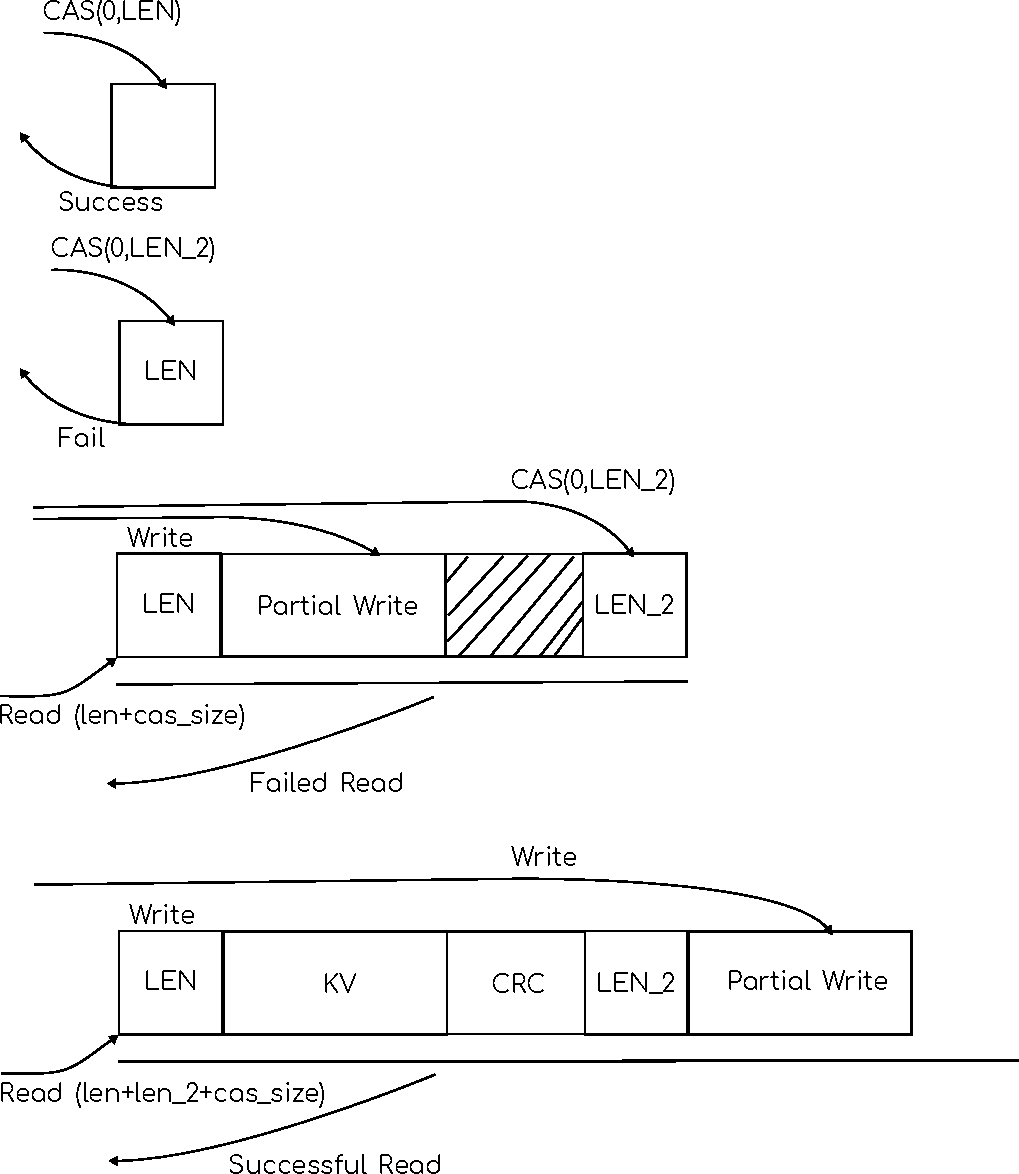
\includegraphics[width=0.485\textwidth]{fig/AppendList.pdf}
%  \vskip -0.5em
%%
\caption{Concurrent operations on write units.}
%%
\label{fig:append_list}
%      \vskip -0.5em
\end{figure}

Figure~\ref{fig:append_list} Illustrates a more complex set of concurrent reads
and writes on write units in sequential memory. In the first operation a client
issues a successful CAS of the entry size to allocate it's location and size. In
the second operation another client attempts the same operation with a different
length, and the operation fails as the allocation has already been made. The
third image shows three concurrent operations. First the client which allocated
with it's CAS in operation 1 proceeds to write into it's allocated buffer. The
client from the second operation re-issules its CAS at a distance of LEN from
it's last attempt, this time succeeding in it's allocation of size LEN\_2. At
the same time a client attempts a read. The read is of size len + the CAS size.
The read must be larger than the entry to tell if it's reading the tail. Here
the read fails for 2 reasons. First the read was incomplete on the first entry
because the write was partially complete, the CRC calculation will fail on the
client. Second the client sees that the following entry has been allocated, and
it has not read enough to determine if the following entry is valid. In the
final example, the write for the second entry is partially completed by the
second writer. The reader reissues a read of size {LEN + LEN\_2 + CAS}. This
time the reader reads the entire first entry, and the second. It sees that the
first is completed, and the second is incomplete, with no following write. In
this case the reader sees the first entry as the valid value for this entry.


\subsection{Hash table index}

\begin{figure}[t] 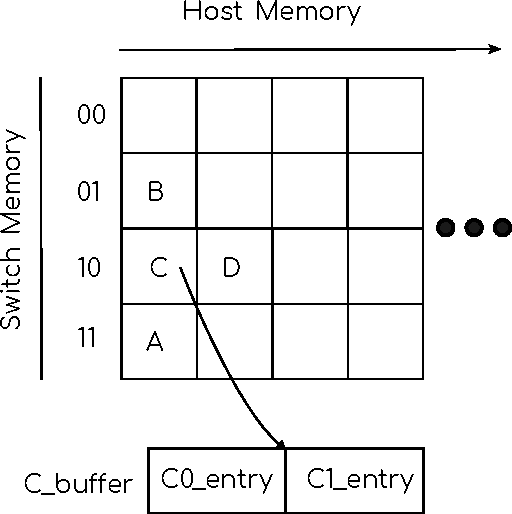
\includegraphics[width=0.485\textwidth]{fig/Index.pdf}
%  \vskip -0.5em

\caption{High level overview of the index. Hash buckets are determined by a hash
prefix. Here 00,01,10,11. On inserts a key is hashed and appended to the bucket
which it lands. Index entries are each write buf entries with a known fixed
size. A switch can track entries per bucket with a counter. Therefore the number
of buckets corresponds to the size of required switch memory. The depth of the
buckets is dependent on the size of host memory.}

\label{fig:index}
%      \vskip -0.5em
\end{figure}

Ideally a hash table index will accept inserts fast, and be quick to look up. To
achieve this we propose a hash table with deep buckets, that contain sequential
elements. A hash table with 4 buckets \textit{00, 01, 10, 11} can hold an
arbitrary number of entries. Each bucket can be allocated to an arbitrary
location in remote memory they need not be sequential. However each bucket must
have a large segment of sequential memory allocated to it.

\textbf{Relaxed Write Units} Each entry in the index is fixed sized, therefore
the requirement that our write unit contain the len of the entry as CAS value
need not be true. We can relax our write unit to only require a CRC and allow
the CAS to contain a pointer to the indexes write value. This saves space, and
allows the insert to be immediately readable prior to finishing the write units
following write.

\textbf{Insert} When an insert occurs a client first allocates a buffer in
remote memory for keys write values. This allocation is outside of the index.
Next the client hashes the key, and appends a write unit pointing to it's write
value into the index. Additional index information such as the key are inserted
into the allocated entry space by a following write. Note that prior to the
write finishing the value is readable. Any reader can traverse the atomically
committed pointer and inspect the writes value without danger.

\textbf{Index Structure} Using write units, rather than 64 bit CAS values as
primitives for the index provides advantages over RACE. First it enables the
full use of the 64 bit address space. Second it enables clients to obtain more
information from the index, such as the true key value (not just a hash). Third
it enables the values written to be arbitrarily sized (RACE supports 255 sizes
only).

\textbf{Conflicting Inserts} When performing an insert the client must first
read the index to determine if a conflicting entry exists. The order of
operations is that the client hashes it's key, reads the index. If the index
exists, the insert is terminated. If the key does not exist the insert is
appended to the bucket. If two inserts occur at the same time, for instance if
an allocate occurs, but they key is not yet written, and another client runs an
insert after the partially written one, the lowest index of the key is always
taken buy subsequent reads and the following key is eventually garbage collected.

\textbf{Potential for Programable switches} This hash structure is designed for
read and write steering. Figure~\cite{fig:Index} shows how the hash size scales
relative to switch memory and host memory. Because the number of buckets can be
easily less than the number of entries a switch must only track the index
counter for each bucket which may be far less than the total number of keys.
Further if each bucket has fixed size entries the switch need only track the
number of entries in the bucket rather than its virtual address. Assuming a max
of 16 entries per bucket this allows for only 4 bits per bucket of metadata on
the switch. Given Tofinio 2 with 20 MB of SRAM this would allow the switch to
handle inserts up to 640 million keys. If we were to allow buckets to become 255
entries deep and use 8 bits per bucket. The switch could support steering up to
40 billion end host keys.

\textbf{Read optimizations} Because the index is append only, and the appends
happen in sequential memory, on search reads can be expanded to capture more of
the index. In the trivial case a read would be a single entry, if th entry is
not the one the client is searching for, it would move to the next like a
typical linked list. Here the client can expand it's read to capture more of the
index in a single round trip, if it is known that the index is loaded. Further
because the switch knows the load of each bucket it can resize the read to the
correct size (or location) to capture the index value it is searching for.

\subsection{Write Buffers} 

Write buffers operate similarly to the index but are for tracking writes to a
single key. Writes and reads are performed like default write units. Writes can
have any size, and are self validating.

\textbf{performing a write} Writes, like inserts first require knowing the index
location. If a write has the index cached, it attempts to write to the end of
the known write list. If it has stale data, it's CAS allocate will fail and it
will proceed to read until it finds the new tail of the write list. When a
successful CAS occurs the writer then fills in the allocation with a write.
Finally the index is update to point to the new write location.

\textbf{batch operations} Colocated clients can batch their operations (ex flat
combining~\cite{flat-combine}) for increased performance. When a CAS is issued
to allocate a write, it can be allocated for multiple entries simply by
increasing the size of the len to multiple entries. Once multiple entries have
been written, the issuing client can resize the len by issuing a second CAS to
the same location but for the size of only the first entry. To save this
additional round trip a header bit could be set on the CAS which indicates to
the reader that the allocation contains multiple entries. This way no round trip
is required, and readers can asynchronously read individual entries as soon as
they complete.

\begin{figure}[t] 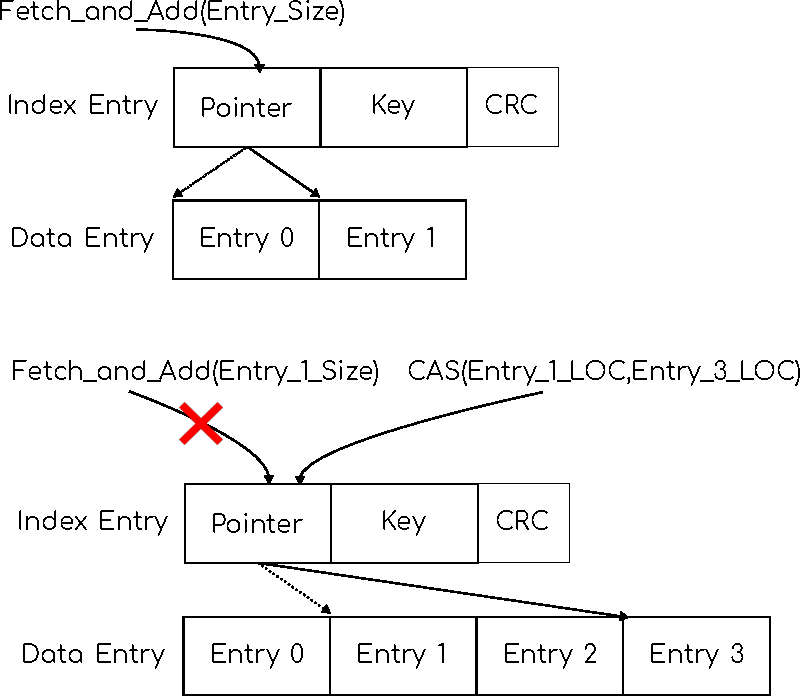
\includegraphics[width=0.485\textwidth]{fig/write_updates.pdf}
%  \vskip -0.5em

\caption{ Unsafe index updates. Fetch-and-Add is used for pointer arithmetic
rather than an explicit pointer update. In the common case Fetch-and-Add adjusts
the pointer correctly. Under failures, or incorrect operation, CAS is a backup
option when inconsistencies occur. (Many corner cases are left as an exercise to
the reader.)}

\label{fig:wait_free_update}
%      \vskip -0.5em
\end{figure}

\textbf{Updating the index on writes} Traditionally an update to the index would
involve reading the old pointer location, then running a CAS(old,new). This same
operation is safe, and can be used to ensure the latest write is easy to find.
Note that we use the index pointer as a hint, and not as a definition of truth.
After locating an index, a concurrent write may make the index invalid.

\textbf{Wait-Free index updates} For speed we could forgo using CAS and instead use
FAA. Because writes are sequential in memory, the len of the prior entry can be
FAA'd to the index pointer. Figure~\ref{wait_free_update} shows the wait-free
algorithm. This ensures that all index updates succeed because FAA is associate
and CAS is not. If concurrent writes result in two FAA being delivered out of
order the sum of the two will still be correct. Therefore the index will
eventually be correct. If a read occurs in an inconsistent state we can use some
sort of identifier in the write to know where the start and end of entries are.
If a client dies before performing an update. Another client can always correct
the index by reading the last entry, locking the writes, and then fixing it with
a CAS.